\documentclass[tikz,border=2mm]{standalone}
\usepackage{amsmath}
\usepackage{fontspec}
\setmainfont{Times New Roman}
\usetikzlibrary{arrows.meta,positioning,shapes.geometric,calc}
\begin{document}
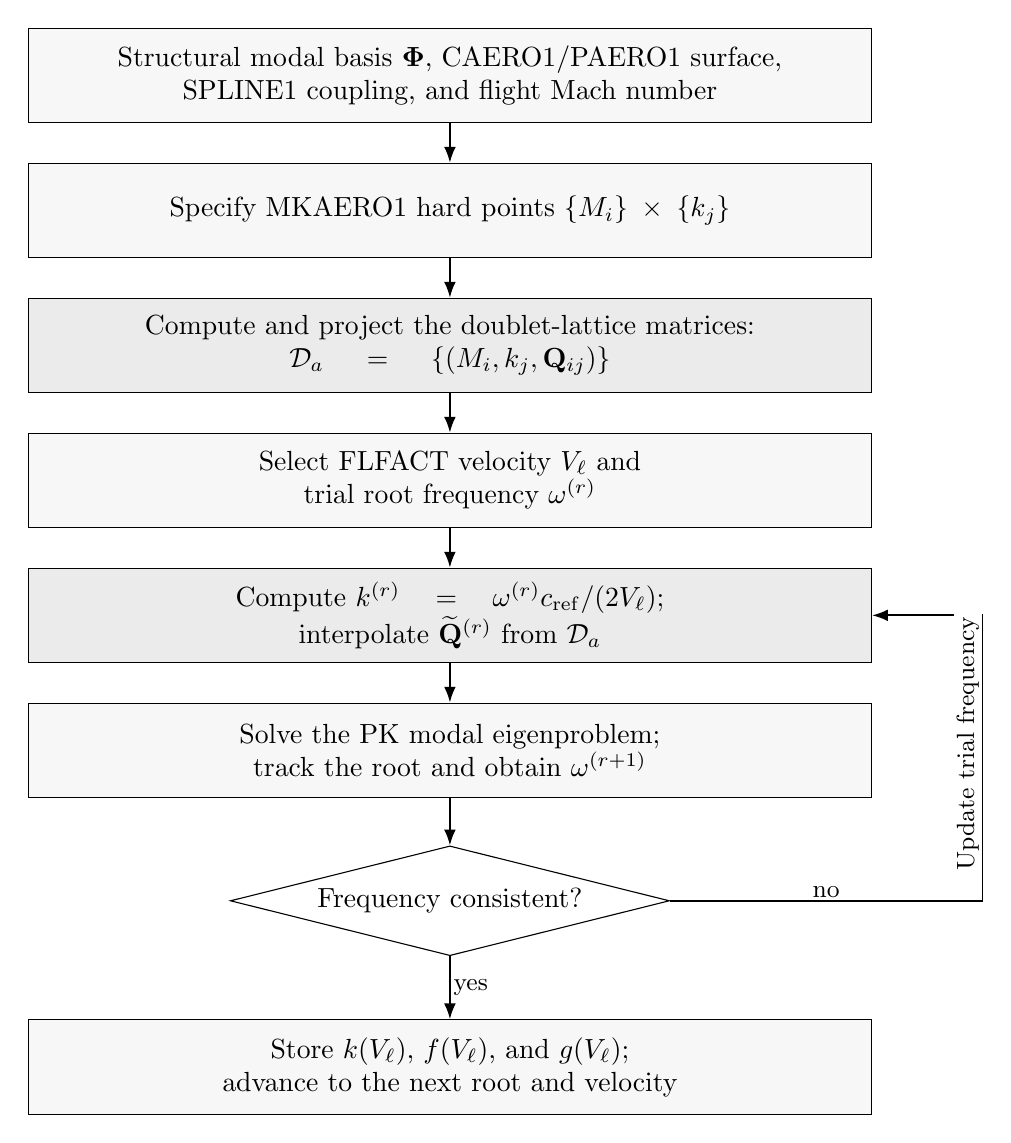
\begin{tikzpicture}[
  >={Latex[length=2mm]},
  every node/.style={font=\fontsize{10}{12}\selectfont,align=center},
  process/.style={draw,fill=black!3,text width=105mm,
    minimum height=12mm,inner sep=3pt},
  database/.style={process,fill=black!8},
  decision/.style={diamond,draw,fill=white,aspect=4,
    text width=38mm,inner sep=1.5pt},
  flow/.style={->,line width=0.65pt},
  note/.style={font=\fontsize{9}{10.5}\selectfont,fill=white,inner sep=1pt}]
  \node[process] (models)
    {Structural modal basis $\boldsymbol{\Phi}$, CAERO1/PAERO1 surface,\\
    SPLINE1 coupling, and flight Mach number};
  \node[process,below=5mm of models] (mkaero)
    {Specify MKAERO1 hard points $\{M_i\}\times\{k_j\}$};
  \node[database,below=5mm of mkaero] (db)
    {Compute and project the doublet-lattice matrices:\\
    $\mathcal{D}_a=\{(M_i,k_j,\mathbf{Q}_{ij})\}$};
  \node[process,below=5mm of db] (trial)
    {Select FLFACT velocity $V_\ell$ and\\
    trial root frequency $\omega^{(r)}$};
  \node[database,below=5mm of trial] (lookup)
    {Compute $k^{(r)}=\omega^{(r)}c_{\mathrm{ref}}/(2V_\ell)$;\\
    interpolate $\widetilde{\mathbf{Q}}^{(r)}$ from $\mathcal{D}_a$};
  \node[process,below=5mm of lookup] (solve)
    {Solve the PK modal eigenproblem;\\
    track the root and obtain $\omega^{(r+1)}$};
  \node[decision,below=6mm of solve] (conv)
    {Frequency consistent?};
  \node[process,below=8mm of conv] (out)
    {Store $k(V_\ell)$, $f(V_\ell)$, and $g(V_\ell)$;\\
    advance to the next root and velocity};

  \draw[flow] (models) -- (mkaero);
  \draw[flow] (mkaero) -- (db);
  \draw[flow] (db) -- (trial);
  \draw[flow] (trial) -- (lookup);
  \draw[flow] (lookup) -- (solve);
  \draw[flow] (solve) -- (conv);
  \draw[flow] (conv) -- node[note,right]{yes} (out);
  \coordinate (lane) at ([xshift=14mm]lookup.east);
  \draw[flow] (conv.east) -- node[note,above]{no}
    (lane |- conv.east) -- (lane) -- (lookup.east);
  \node[note,rotate=90,above=1.8mm] at ($(lane)!0.5!(lane |- conv.east)$)
    {Update trial frequency};
\end{tikzpicture}
\end{document}
